\documentclass[a4paper, utf8]{ctexart}
\usepackage[fontset=Fandol]{ctex}
\usepackage{anyfontsize}
\usepackage{algorithm}
\usepackage{longtable}
\usepackage{abstract}
\usepackage{amsfonts}
\usepackage{appendix}
\usepackage{booktabs}
\usepackage{enumitem}
\usepackage{fancyhdr}
\usepackage{geometry}
\usepackage{graphicx}
\usepackage{tabularx}
\usepackage{listings}
\usepackage{amsmath}
\usepackage{caption}
\usepackage{lipsum}
\usepackage{minted}
\usepackage{xcolor}
\usepackage{array}

\geometry{a4paper,left=31mm,right=31mm,top=25mm,bottom=25mm}
\CTEXsetup[format={\Large \bfseries}]{section}

\setlength{\parindent}{2em}
\pagestyle{fancy}
\fancyhf{}
\fancyhead[L]{并行程序设计与算法实验\ 实验报告}
\fancyhead[R]{Lab5\ 基于OpenMP的并行矩阵乘法}
\fancyhead[C]{}
\fancyfoot[C]{\thepage}
\fancyfoot[L,R]{}

\setCJKfamilyfont{zhsong}[AutoFakeBold = {2.17}]{SimSun}
\renewcommand*{\songti}{\CJKfamily{zhsong}}
\definecolor{LightGray}{gray}{0.9}

\title{\songti \bfseries Lab5\ 基于OpenMP的并行矩阵乘法}
\author{\fangsong 21307210\ \ 傅祉珏}
\date{\fangsong 中山大学计算机学院\ 广东广州\ 510006}

\begin{document}
	
	\begin{titlepage}
		\centering
		\rule{\textwidth}{1pt}
		\vspace{0.02\textheight}
		
		{\LARGE \kaishu 并行程序设计与算法实验\ 实验报告}
		
		\vspace{0.02\textheight}
		
		{\huge \songti \bfseries Lab5\ 基于OpenMP的并行矩阵乘法}
		
		\vspace{0.025\textheight}
		\rule{0.83\textwidth}{0.4pt}
		\vspace{0.05\textheight} 
		\begin{figure}[htbp]
			\centering
			
\includegraphics[width=8cm, height=8cm]{./figure/计院院徽.jpg}
		\end{figure}
		
		\vspace{0.04\textheight} 
		{\Large 姓名:傅祉珏}
		
		\vspace{0.025\textheight} 
		{\Large 学号:21307210}
		
		\vspace{0.025\textheight} 
		{\Large 专业:计算机科学与技术}
		
		\vspace{0.025\textheight} 
		{\Large Email:futk@mail2.sysu.edu.cn}
		
		\vspace{0.025\textheight} 
		{\Large 完成时间:\today}
		
		\vspace{0.05\textheight} 
		\vfill
		
		{\large \today}
		\vspace{0.1\textheight}
		\rule{\textwidth}{1pt}
	\end{titlepage}
	\let\cleardoublepage\clearpage
	
	\maketitle
	
	\renewcommand{\abstractname}{\large \textbf{摘要}}
	\begin{abstract}
		本实验旨在通过OpenMP实现并行通用矩阵乘法(GEMM),系统考察线程数量、矩阵规模和调度策略对并行性能的影响。实验设计了从$128\times128$到$2048\times2048$的多组矩阵规模,分别在默认、静态与动态三种调度方式下,结合不同线程数量进行测试与时间测量。结果表明,随着矩阵规模的增大,静态调度(\verb|static|)在运行时间与效率上优于默认(\verb|default|)与动态(\verb|dynamic|)调度,尤其在中大型矩阵乘法中表现突出。动态调度在小规模任务中因调度开销导致性能下降,而默认调度整体表现介于两者之间。实验进一步揭示了线程竞争、内存带宽瓶颈等硬件资源因素对并行加速效果的制约。通过本实验,掌握了基于OpenMP的并行任务划分、线程管理及调度优化的方法,为后续高性能计算应用奠定了实践基础。
		
		\noindent{\textbf{\heiti 关键词:}OpenMP,并行矩阵乘法,调度策略,性能优化,线程管理。}
	\end{abstract}
	
	\section{实验目的}
	
	在本实验中,旨在通过基于OpenMP的多线程编程实现并行通用矩阵乘法(General Matrix Multiplication, GEMM),加深对并行计算基本原理与实践方法的理解。实验任务要求随机生成两个矩阵,分别为尺寸为$m \times n$的矩阵A和尺寸为$n \times k$的矩阵B,执行标准矩阵乘法运算以计算出$m \times k$的结果矩阵C,并记录矩阵计算所消耗的时间。实验过程中,将系统地调整多个关键参数,包括线程数量(1至16个)、矩阵规模(从128到2048的不同取值),以及OpenMP提供的多种调度机制(默认调度、静态调度与动态调度),以全面考察不同配置下程序的并行性能表现。
	
	通过本实验,学生将深入理解OpenMP并行模型中任务划分、线程管理和负载均衡的实现机制,掌握利用并行指令(如\verb|#pragma omp parallel for|)加速计算密集型任务的方法,并能够根据不同的应用场景合理选择和优化调度策略。同时,通过对实验数据的分析比较,进一步培养评估程序性能(如加速比、效率)及分析性能瓶颈的能力。实验还将帮助学生认识到硬件资源(如CPU核心数)对并行计算性能的影响,为今后在高性能计算(HPC)、科学计算及工程应用中设计高效并行算法打下坚实基础。
	
	\section{实验过程}
	
	在本实验中,为实现基于OpenMP的并行矩阵乘法运算,首先编写了矩阵生成函数\verb|gener|\ \verb|ate_matrix|,用于初始化输入矩阵$A$和$B$。该函数通过随机数生成器为矩阵中的每个元素赋值,生成值域在$0$到$10$之间的浮点数,保证了实验数据的多样性和广泛适用性。随后设计了矩阵乘法核心函数\verb|matrix_multiply|,在该函数内部采用OpenMP并行化技术,将矩阵元素的计算任务划分至不同线程中执行。具体地,使用了\verb|#pragma omp parallel for collapse(2)|\ \verb|schedule(runtime)|指令,实现对矩阵元素双重循环($i$和$j$方向)的并行展开,并通过OpenMP运行时调度策略管理任务分配。
	
	\begin{minted}[baselinestretch=1, framesep=0mm, escapeinside=||]{cpp}
void matrix_multiply(double* A, double* B, double* C, int m, int n, int k, 
                     int num_threads, int schedule_mode) {
    omp_set_num_threads(num_threads);

    #pragma omp parallel for collapse(2) schedule(runtime)
    for (int i = 0; i < m; i++) {
        for (int j = 0; j < k; j++) {
            double sum = 0.0;
            for (int l = 0; l < n; l++) {
                sum += A[i * n + l] * B[l * k + j];
            }
            C[i * k + j] = sum;
        }
    }
}
	\end{minted}
	
	在主程序部分,依次设定了$16$组不同规模的矩阵,其尺寸从$128\times128$递增至$2048\times2048$,覆盖了从小规模到大规模计算任务的全范围。对于每一组矩阵规模,程序分别测试了三种不同的调度策略:默认调度(不显式设置)、静态调度(\verb|omp_sched_static|)和动态调度(\verb|omp_sched_dynamic|)。在每种调度策略下,进一步设置线程数从$1$到$16$进行测试,系统性地收集在不同线程数量条件下的执行时间数据。时间测量使用了OpenMP提供的高精度计时函数\verb|omp_get_wtime()|,确保实验结果的准确性与可比性。
	
	\begin{minted}[baselinestretch=1, framesep=0mm, escapeinside=||]{cpp}
for (int s = 0; s < 3; s++) {
    printf("\nSchedule Mode: %s\n", schedule_names[s]);
    for (int t = 0; t < 16; t++) {
        int num_threads = thread_counts[t];

        if (s == 1) omp_set_schedule(omp_sched_static, 0);
        else if (s == 2) omp_set_schedule(omp_sched_dynamic, 0);
        else /* default: do not set */;

        double start_time = omp_get_wtime();
        matrix_multiply(A, B, C, m, n, k, num_threads, s);
        double end_time = omp_get_wtime();

        printf("Threads: %d, Time: %.2f ms\n", num_threads, (end_time - 
                start_time) * 1000);
    }
}
	\end{minted}
	
	实验过程中,为保证结果的正确性与稳定性,每轮测试均在生成新矩阵A和B后进行完整的矩阵乘法计算,并在计算结束后及时释放分配的内存资源,防止内存泄漏问题。同时,考虑到大规模矩阵的输出不便展示,屏蔽了中间矩阵打印函数\verb|print_matrix|,以专注于性能测试。通过上述设置,本实验能够充分比较在不同矩阵规模、不同线程数量和不同调度模式下,基于OpenMP的并行矩阵乘法实现的性能变化规律,为后续的性能分析与优化提供了详实的数据支撑。
	
	\section{实验结果}
	
	在本次实验中,我们针对不同规模的矩阵(从$128\times128$到$2048\times2048$)进行了并行矩阵乘法计算,比较了OpenMP默认调度、\verb|static|调度与\verb|dynamic|调度三种方式下的执行时间表现。实验结果表明,随着矩阵规模的增大,三种调度策略在运行时间上的差异也逐渐显现。在小规模矩阵(如$128$、$256$)的计算中,三种调度方式差别不大,且整体运行时间非常短,通常在几毫秒以内,\verb|dynamic|调度略慢于\verb|default|和\verb|static|调度,这可能是因为\verb|dynamic|在小任务量时调度开销较大,反而影响了整体效率。
	
	\begin{figure}[htbp]
		\centering
		\begin{minipage}{.32\textwidth}
			\centering
			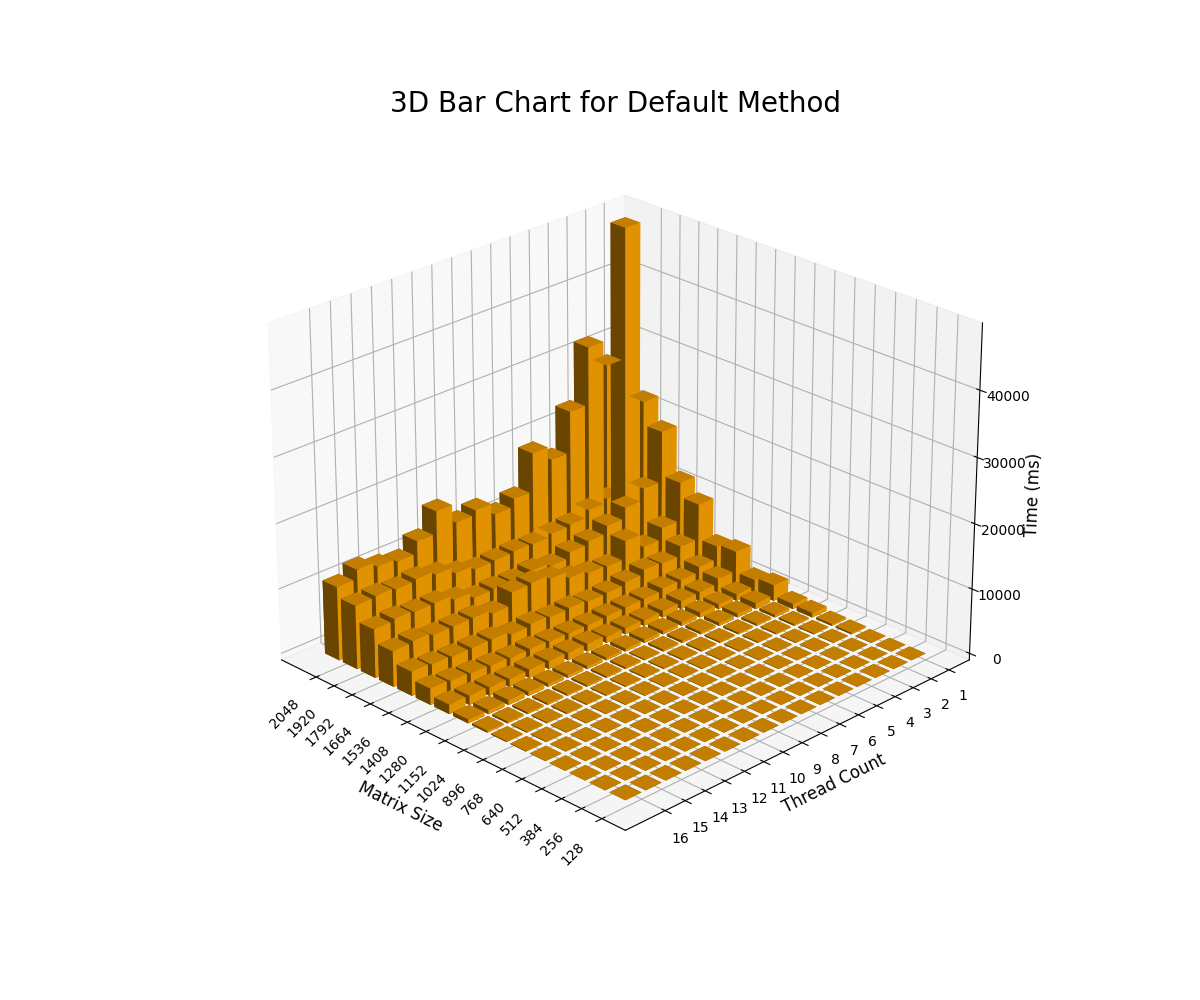
\includegraphics[width=.8\textwidth]{./figure/default_barchart.png}
			\caption{默认调度性能图}
		\end{minipage}
		\begin{minipage}{.32\textwidth}
			\centering
			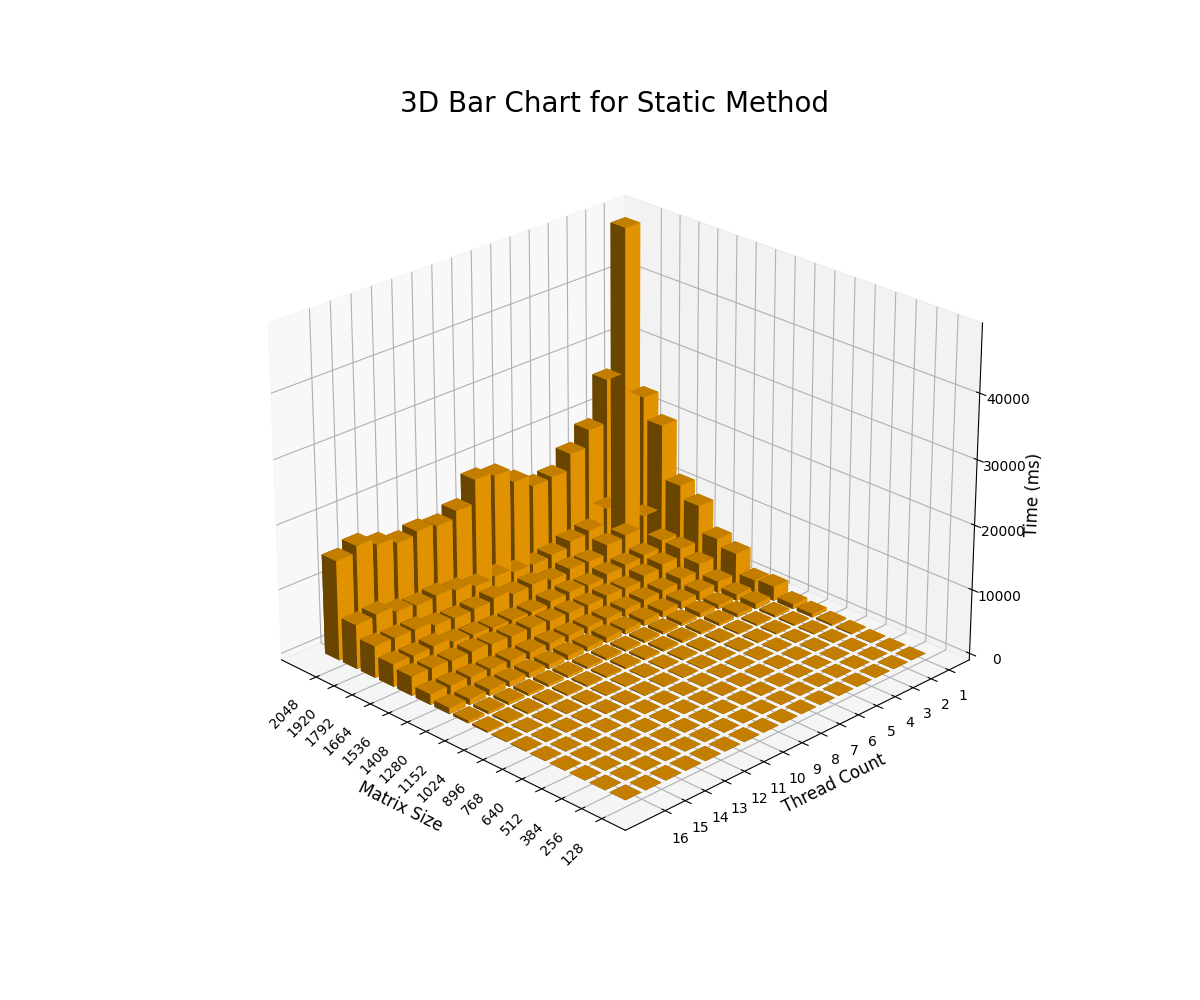
\includegraphics[width=.8\textwidth]{./figure/static_barchart.png}
			\caption{静态调度性能图}
		\end{minipage}
		\begin{minipage}{.32\textwidth}
			\centering
			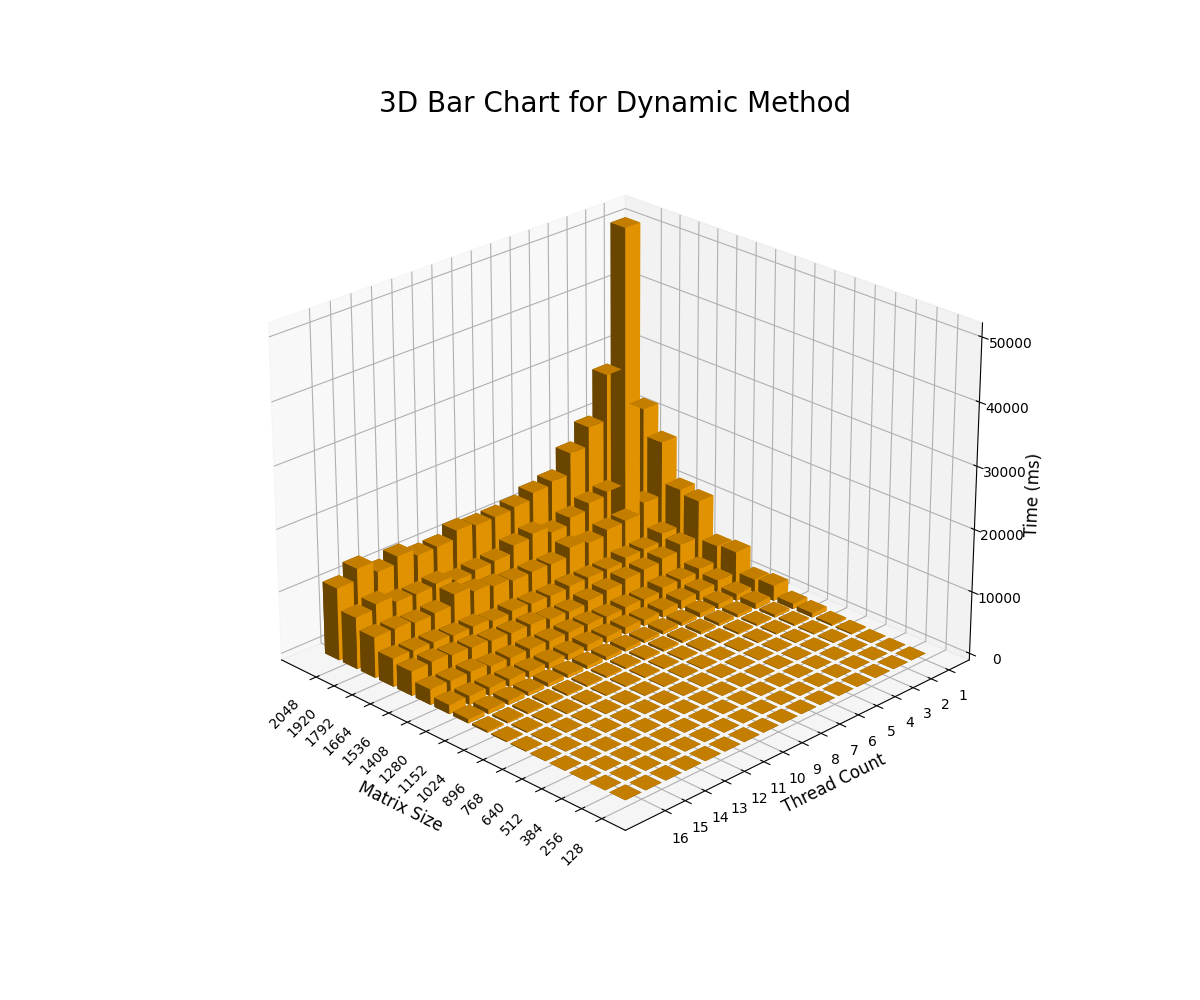
\includegraphics[width=.8\textwidth]{./figure/dynamic_barchart.png}
			\caption{动态调度性能图}
		\end{minipage}
	\end{figure}
	
	当矩阵规模逐步扩大到$512$及以上时,\verb|static|调度开始展现出明显的优势。无论是在$512$、$768$还是$1024$的规模下,\verb|static|调度通常能比\verb|default|和\verb|dynamic|获得更低的运行时间。例如,在$1024\times1024$矩阵的计算中,\verb|static|调度通常比\verb|default|减少了约$20\%$至$30\%$的计算时间,而\verb|dynamic|调度则表现出较高的波动性,个别情况下甚至比\verb|default|还要慢。这表明\verb|static|调度在负载较均匀、计算密集型的矩阵乘法场景下,能更有效地减少线程空闲和调度开销,从而提高整体并行效率。
	
	进一步增大矩阵规模至$1536$、$1792$、$2048$时,实验数据同样验证了\verb|static|调度的优势。尽管随着规模的扩大,总运行时间显著上升,最高达到数万毫秒,但\verb|static|调度在大部分样本中仍然保持了相对较低的耗时。而\verb|dynamic|调度尽管在某些大规模样本中可以应对轻微的不均衡负载,提升局部性能,但整体来看其调度开销在大规模矩阵乘法中仍然偏高,不如\verb|static|调度高效。\verb|default|调度的性能则介于\verb|static|与\verb|dynamic|之间,表现较为中规中矩。
	
	综合实验过程和结果可以得出结论:在矩阵乘法这种计算负载均匀、任务划分简单的应用中,使用OpenMP的\verb|static|调度策略可以显著提升并行计算的性能。而\verb|dynamic|调度更适用于负载不均、任务复杂度差异较大的情形,在本实验中并不占优。\verb|default|调度虽然能自动根据OpenMP实现选择适合的策略,但在特定任务(如矩阵乘法)中,显式选择\verb|static|调度可以获得更好的效果。因此,合理选择并行调度策略对提升OpenMP程序的性能具有重要意义。
	
	\begin{figure}[htbp]
		\centering
		\begin{minipage}{.45\textwidth}
			\centering
			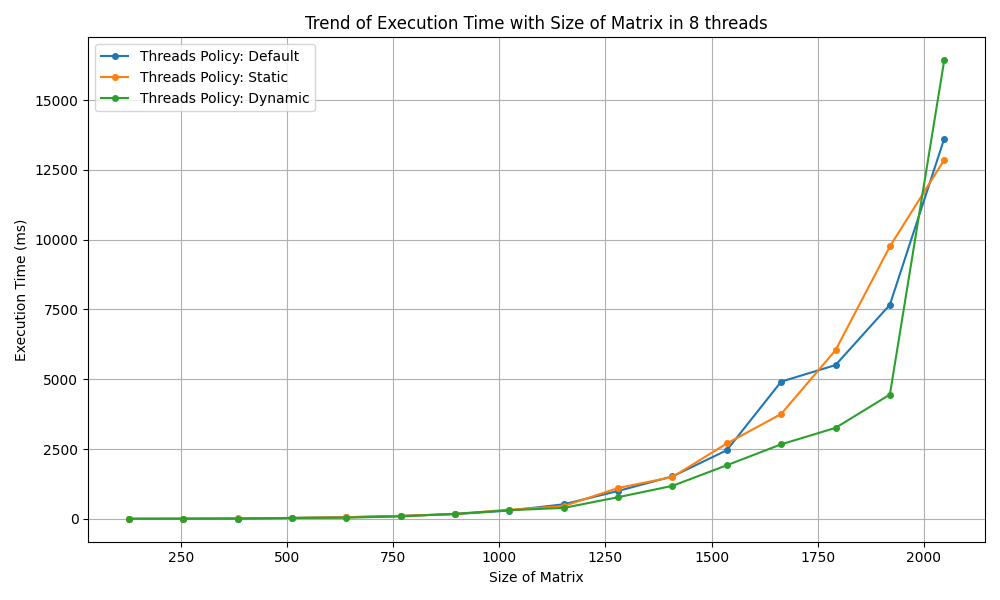
\includegraphics[width=.8\textwidth]{./figure/method_time_trend.png}
			\caption{调度方式性能对比图}
		\end{minipage}
		\begin{minipage}{.45\textwidth}
			\centering
			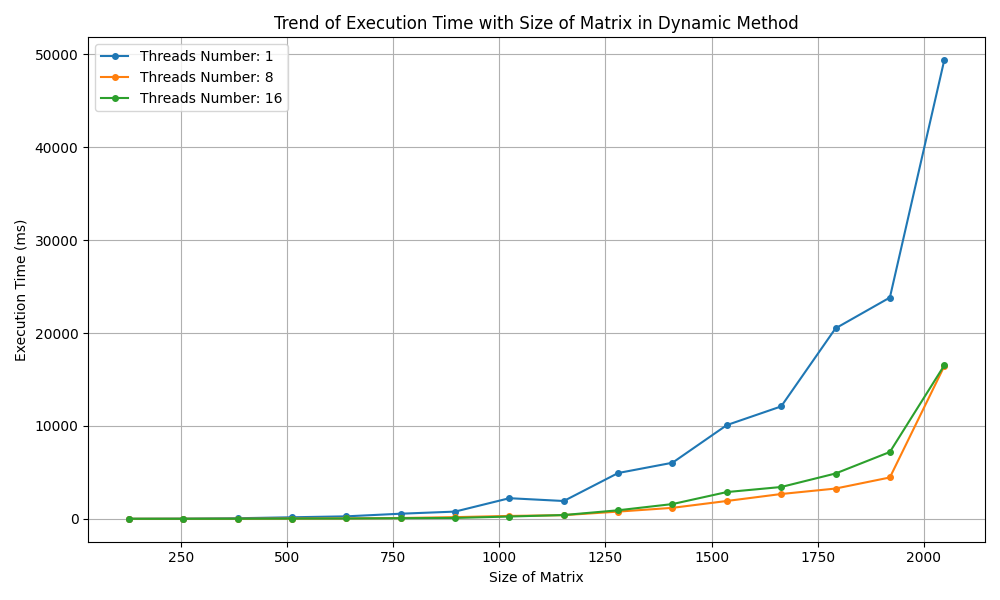
\includegraphics[width=.8\textwidth]{./figure/threads_time_trend.png}
			\caption{线程数性能对比图}
		\end{minipage}
	\end{figure}
	
	值得注意的是,在使用更多线程并行运行时,虽然整体趋势仍是并行执行优于串行执行,但在部分测试中观察到性能出现波动甚至下降,尤其是动态调度下尤为明显。出现这种现象的原因主要有两方面:一是线程间存在更频繁的竞争与同步开销,当任务粒度过细或线程数量过多时,调度和上下文切换的负担加重,反而削弱了并行的优势;二是系统资源(如内存带宽、缓存容量)受限,多个线程同时访问大矩阵数据时,会导致缓存未命中率上升,增加主存访问延迟,从而使得总体执行效率下降。
	
	\section{总结与思考}
	
	通过本次基于OpenMP的并行矩阵乘法实验,我们深入分析了不同线程数量、矩阵规模及调度策略对并行性能的影响,得出了一些有价值的结论。首先,在矩阵乘法这一计算负载均匀、任务划分规律的应用场景中,使用静态(\verb|static|)调度能够更好地发挥OpenMP并行加速的优势。与默认(\verb|default|)和动态(\verb|dynamic|)调度相比,静态调度在中大规模矩阵(如$512\times512$及以上)计算中表现出更低的运行时间和更高的效率,说明在负载均衡、调度开销可控的前提下,静态划分能够最大程度减少线程空闲与调度成本,提高资源利用率。
	
	此外,实验中也观察到随着线程数量的增加,程序性能并非始终线性提升。在某些情况下,增加线程数反而导致了性能下降,尤其是在采用动态调度时更为显著。这种现象主要源于两个方面:一方面,线程之间的竞争与同步开销随着线程数上升而增大,当任务粒度不足够大时,频繁的任务切换和上下文管理反而带来额外负担,削弱了并行带来的速度提升;另一方面,系统硬件资源(如内存带宽、缓存容量)存在瓶颈,多个线程在大矩阵运算中同时访问共享数据,导致缓存未命中率上升,访问主存的延迟显著增加,从而使得整体执行效率下降。这一发现强调了在并行编程中合理控制线程数量、平衡任务粒度与同步成本的重要性。
	
	综上所述,本实验验证了调度策略选择和线程管理对并行性能的显著影响,进一步认识到并行化并非线程越多越好,而需要结合具体应用特性与硬件环境,合理优化任务划分与资源调度,才能真正发挥出高性能计算的潜力。
	
	\let\cleardoublepage\clearpage
	
	\begin{thebibliography}{99}  
		\bibitem{ref1} 彼得·S·帕切科,\ 马修·马伦塞克.\ 并行程序设计导论[M].\ 黄智濒,\ 肖晨\ 译.\ 原书第2版.\ 北京:机械工业出版社,\ 2024.
		\bibitem{ref2} 黄聃.\ 课件5[EB/OL].\ [2025-3-10].\ https://easyhpc.net/course/221/lesson/1416/material/3173.
		\bibitem{ref3} 黄聃.\ 课件6[EB/OL].\ [2025-3-10].\ https://easyhpc.net/course/221/lesson/1450/material/3182.
	\end{thebibliography}
	
\end{document}
